\documentclass{standalone}
\usepackage{tikz}
\usetikzlibrary{patterns, positioning}
\usepackage[sfdefault]{ClearSans} %% option 'sfdefault' activates Clear Sans as the default text font
\usepackage[T1]{fontenc}

\begin{document}
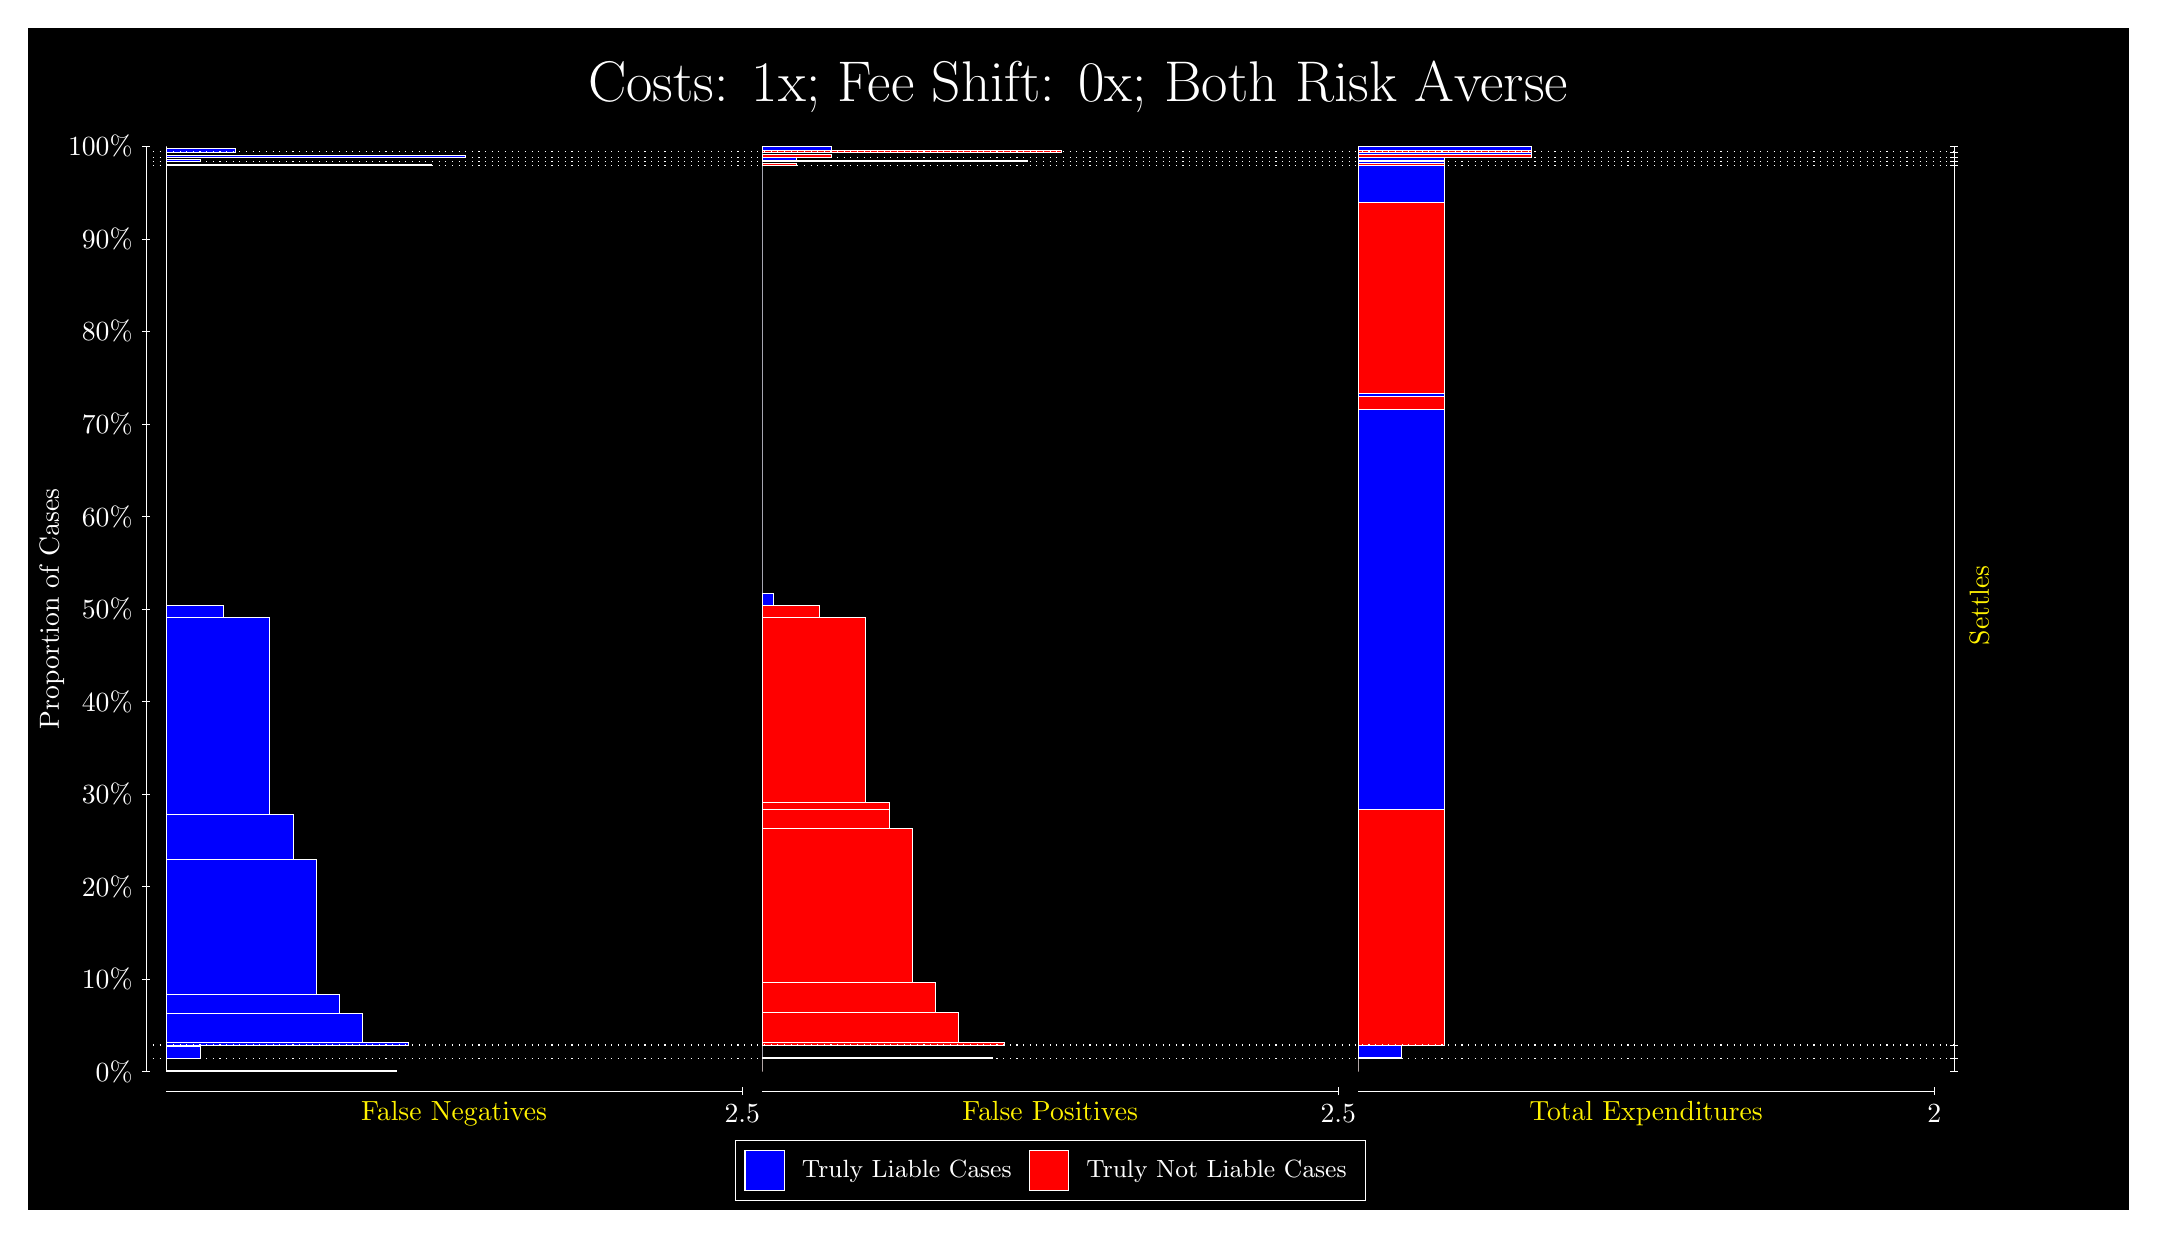
\begin{tikzpicture}
\draw[fill=black] (0,0) rectangle (26.667,15);
\draw[text=white] (0,13.5) rectangle (26.667,15) node[midway] {\huge Costs: 1x; Fee Shift: 0x; Both Risk Averse};
\draw[white, very thin] (1.5,1.75) -- (1.5,13.5);
\node[rotate=90, text=white, anchor=center] at (0.3, 7.625) {Proportion of Cases};
\draw[white, very thin] (1.45,1.75) -- (1.55,1.75);
\node[text=white, anchor=east] at (1.45, 1.75) {0\%};
\draw[white, very thin] (1.45,2.925) -- (1.55,2.925);
\node[text=white, anchor=east] at (1.45, 2.925) {10\%};
\draw[white, very thin] (1.45,4.1) -- (1.55,4.1);
\node[text=white, anchor=east] at (1.45, 4.1) {20\%};
\draw[white, very thin] (1.45,5.275) -- (1.55,5.275);
\node[text=white, anchor=east] at (1.45, 5.275) {30\%};
\draw[white, very thin] (1.45,6.45) -- (1.55,6.45);
\node[text=white, anchor=east] at (1.45, 6.45) {40\%};
\draw[white, very thin] (1.45,7.625) -- (1.55,7.625);
\node[text=white, anchor=east] at (1.45, 7.625) {50\%};
\draw[white, very thin] (1.45,8.8) -- (1.55,8.8);
\node[text=white, anchor=east] at (1.45, 8.8) {60\%};
\draw[white, very thin] (1.45,9.975) -- (1.55,9.975);
\node[text=white, anchor=east] at (1.45, 9.975) {70\%};
\draw[white, very thin] (1.45,11.15) -- (1.55,11.15);
\node[text=white, anchor=east] at (1.45, 11.15) {80\%};
\draw[white, very thin] (1.45,12.325) -- (1.55,12.325);
\node[text=white, anchor=east] at (1.45, 12.325) {90\%};
\draw[white, very thin] (1.45,13.5) -- (1.55,13.5);
\node[text=white, anchor=east] at (1.45, 13.5) {100\%};

\draw[white, very thin] (24.457,1.75) -- (24.457,13.5);
\draw[white, very thin] (24.407,1.75) -- (24.507,1.75);
\node[anchor=west] at (24.407, 1.75) {};
\draw[white, very thin] (24.407,1.9182) -- (24.507,1.9182);
\node[anchor=west] at (24.407, 1.9182) {};
\draw[white, very thin] (24.407,2.0863) -- (24.507,2.0863);
\node[anchor=west] at (24.407, 2.0863) {};
\draw[white, very thin] (24.407,13.257) -- (24.507,13.257);
\node[anchor=west] at (24.407, 13.257) {};
\draw[white, very thin] (24.407,13.305) -- (24.507,13.305);
\node[anchor=west] at (24.407, 13.305) {};
\draw[white, very thin] (24.407,13.359) -- (24.507,13.359);
\node[anchor=west] at (24.407, 13.359) {};
\draw[white, very thin] (24.407,13.429) -- (24.507,13.429);
\node[anchor=west] at (24.407, 13.429) {};
\draw[white, very thin] (24.407,13.5) -- (24.507,13.5);
\node[anchor=west] at (24.407, 13.5) {};

\draw[white, very thin, fill=blue] (1.75,1.75) rectangle (4.6775,1.7677);
\draw[white, very thin, fill=red] (1.75,1.7677) rectangle (1.75,1.9182);
\draw[white, very thin, fill=blue] (1.75,1.9182) rectangle (2.1891,2.0687);
\draw[white, very thin, fill=red] (1.75,2.0687) rectangle (1.75,2.0863);
\draw[white, very thin, fill=blue] (1.75,2.0863) rectangle (4.8239,2.1207);
\draw[white, very thin, fill=blue] (1.75,2.1207) rectangle (4.2384,2.4852);
\draw[white, very thin, fill=blue] (1.75,2.4852) rectangle (3.9457,2.7257);
\draw[white, very thin, fill=blue] (1.75,2.7257) rectangle (3.6529,4.4459);
\draw[white, very thin, fill=blue] (1.75,4.4459) rectangle (3.3602,5.0177);
\draw[white, very thin, fill=blue] (1.75,5.0177) rectangle (3.0674,7.5135);
\draw[white, very thin, fill=blue] (1.75,7.5135) rectangle (2.4819,7.6703);
\draw[white, very thin, fill=red] (1.75,7.6703) rectangle (1.75,13.257);
\draw[white, very thin, fill=blue] (1.75,13.257) rectangle (5.1167,13.277);
\draw[white, very thin, fill=red] (1.75,13.277) rectangle (1.75,13.305);
\draw[white, very thin, fill=blue] (1.75,13.305) rectangle (2.1891,13.336);
\draw[white, very thin, fill=red] (1.75,13.336) rectangle (1.75,13.359);
\draw[white, very thin, fill=blue] (1.75,13.359) rectangle (5.5558,13.383);
\draw[white, very thin, fill=red] (1.75,13.383) rectangle (1.75,13.429);
\draw[white, very thin, fill=blue] (1.75,13.429) rectangle (2.6283,13.476);
\draw[white, very thin, fill=red] (1.75,13.476) rectangle (1.75,13.5);
\draw[white, very thin, fill=red] (9.3189,1.75) rectangle (9.3189,1.9005);
\draw[white, very thin, fill=blue] (9.3189,1.9005) rectangle (9.3189,1.9182);
\draw[white, very thin, fill=red] (9.3189,1.9182) rectangle (12.246,1.9359);
\draw[white, very thin, fill=blue] (9.3189,1.9359) rectangle (9.3189,2.0863);
\draw[white, very thin, fill=red] (9.3189,2.0863) rectangle (12.393,2.1207);
\draw[white, very thin, fill=red] (9.3189,2.1207) rectangle (11.807,2.5003);
\draw[white, very thin, fill=red] (9.3189,2.5003) rectangle (11.515,2.8794);
\draw[white, very thin, fill=red] (9.3189,2.8794) rectangle (11.222,4.8383);
\draw[white, very thin, fill=red] (9.3189,4.8383) rectangle (10.929,5.083);
\draw[white, very thin, fill=red] (9.3189,5.083) rectangle (10.929,5.1656);
\draw[white, very thin, fill=red] (9.3189,5.1656) rectangle (10.636,7.5161);
\draw[white, very thin, fill=red] (9.3189,7.5161) rectangle (10.051,7.6729);
\draw[white, very thin, fill=blue] (9.3189,7.6729) rectangle (9.4652,7.8298);
\draw[white, very thin, fill=blue] (9.3189,7.8298) rectangle (9.3189,13.257);
\draw[white, very thin, fill=red] (9.3189,13.257) rectangle (9.758,13.284);
\draw[white, very thin, fill=blue] (9.3189,13.284) rectangle (9.3189,13.305);
\draw[white, very thin, fill=red] (9.3189,13.305) rectangle (12.686,13.327);
\draw[white, very thin, fill=blue] (9.3189,13.327) rectangle (9.758,13.359);
\draw[white, very thin, fill=red] (9.3189,13.359) rectangle (10.197,13.405);
\draw[white, very thin, fill=blue] (9.3189,13.405) rectangle (9.3189,13.429);
\draw[white, very thin, fill=red] (9.3189,13.429) rectangle (13.125,13.454);
\draw[white, very thin, fill=blue] (9.3189,13.454) rectangle (10.197,13.5);
\draw[white, very thin, fill=red] (16.888,1.75) rectangle (16.888,1.9005);
\draw[white, very thin, fill=blue] (16.888,1.9005) rectangle (16.888,1.9182);
\draw[white, very thin, fill=red] (16.888,1.9182) rectangle (17.437,1.9359);
\draw[white, very thin, fill=blue] (16.888,1.9359) rectangle (17.437,2.0863);
\draw[white, very thin, fill=red] (16.888,2.0863) rectangle (17.986,5.083);
\draw[white, very thin, fill=blue] (16.888,5.083) rectangle (17.986,10.166);
\draw[white, very thin, fill=red] (16.888,10.166) rectangle (17.986,10.323);
\draw[white, very thin, fill=blue] (16.888,10.323) rectangle (17.986,10.358);
\draw[white, very thin, fill=red] (16.888,10.358) rectangle (17.986,12.791);
\draw[white, very thin, fill=blue] (16.888,12.791) rectangle (17.986,13.257);
\draw[white, very thin, fill=red] (16.888,13.257) rectangle (17.986,13.284);
\draw[white, very thin, fill=blue] (16.888,13.284) rectangle (17.986,13.305);
\draw[white, very thin, fill=red] (16.888,13.305) rectangle (17.986,13.327);
\draw[white, very thin, fill=blue] (16.888,13.327) rectangle (17.986,13.359);
\draw[white, very thin, fill=red] (16.888,13.359) rectangle (19.083,13.405);
\draw[white, very thin, fill=blue] (16.888,13.405) rectangle (19.083,13.429);
\draw[white, very thin, fill=red] (16.888,13.429) rectangle (19.083,13.454);
\draw[white, very thin, fill=blue] (16.888,13.454) rectangle (19.083,13.5);
\draw[white, dotted] (1.5,1.9182) -- (24.457,1.9182);
\draw[white, dotted] (1.5,2.0863) -- (24.457,2.0863);
\draw[white, dotted] (1.5,13.257) -- (24.457,13.257);
\draw[white, dotted] (1.5,13.305) -- (24.457,13.305);
\draw[white, dotted] (1.5,13.359) -- (24.457,13.359);
\draw[white, dotted] (1.5,13.429) -- (24.457,13.429);
\draw[white, very thin] (1.75,1.5) -- (9.0689,1.5);
\node[text=yellow, anchor=north] at (5.4094, 1.5) {False Negatives};
\draw[white, very thin] (9.0689,1.45) -- (9.0689,1.55);
\node[text=white, anchor=north] at (9.0689, 1.45) {2.5};

\draw[white, very thin] (9.3189,1.5) -- (16.638,1.5);
\node[text=yellow, anchor=north] at (12.978, 1.5) {False Positives};
\draw[white, very thin] (16.638,1.45) -- (16.638,1.55);
\node[text=white, anchor=north] at (16.638, 1.45) {2.5};

\draw[white, very thin] (16.888,1.5) -- (24.207,1.5);
\node[text=yellow, anchor=north] at (20.547, 1.5) {Total Expenditures};
\draw[white, very thin] (24.207,1.45) -- (24.207,1.55);
\node[text=white, anchor=north] at (24.207, 1.45) {2};



\node[text=yellow, centered, rotate=90] at (24.777, 7.6716) {Settles};





\draw (12.978300999999998,1.5) node[draw=none] (baseCoordinate) {};
\begin{scope}[align=center]
        \matrix[scale=0.5, draw=white, below=0.5cm of baseCoordinate, nodes={draw}, column sep=0.1cm]{
            \node[rectangle, draw, minimum width=0.5cm, minimum height=0.5cm, fill=blue] {}; &
            \node[draw=none, font=\small, text=white] (B) {Truly Liable Cases}; &
            \node[rectangle, draw, minimum width=0.5cm, minimum height=0.5cm, fill=red] {}; &
            \node[draw=none, font=\small, text=white] (B) {Truly Not Liable Cases}; \\
            };
\end{scope}

\end{tikzpicture}
\end{document}